\documentclass[11pt,a4paper]{article}

% shared/macros.tex
% Shared notation for all surface-partition math documents.
% Include with: % shared/macros.tex
% Shared notation for all surface-partition math documents.
% Include with: % shared/macros.tex
% Shared notation for all surface-partition math documents.
% Include with: \input{../shared/macros}

% -------------------------------------------------------------------------
% Packages (include here so each document only needs \input{../shared/macros})
% -------------------------------------------------------------------------
\usepackage{amsmath,amssymb,amsthm}
\usepackage{bm}           % \bm for bold math
\usepackage{mathtools}    % \coloneqq, dcases, etc.
\usepackage{booktabs}     % \toprule etc. in tables
\usepackage{hyperref}
\usepackage{geometry}
\usepackage{microtype}
\usepackage{parskip}
\usepackage{xcolor}
\usepackage{tcolorbox}
\usepackage{enumitem}
\usepackage{float}             % [H] float placement

\geometry{a4paper, margin=2.5cm}

% -------------------------------------------------------------------------
% Theorem-like environments
% -------------------------------------------------------------------------
\theoremstyle{definition}
\newtheorem{defn}{Definition}[section]
\newtheorem{remark}{Remark}[section]

\theoremstyle{plain}
\newtheorem{prop}{Proposition}[section]

% -------------------------------------------------------------------------
% Mesh and geometry
% -------------------------------------------------------------------------
\newcommand{\V}{\mathbf{V}}            % vertex array V[i] in R^dim
\newcommand{\F}{\mathbf{F}}            % face (triangle) array
\newcommand{\vone}[1]{v_{1,#1}}       % first vertex index of VP i
\newcommand{\vtwo}[1]{v_{2,#1}}       % second vertex index of VP i

% -------------------------------------------------------------------------
% Variable points
% -------------------------------------------------------------------------
\newcommand{\lam}{\lambda}             % scalar VP parameter
\newcommand{\Lam}{\boldsymbol{\lambda}}% full parameter vector
\newcommand{\vp}[1]{\mathbf{p}_{#1}}  % 3D position of VP i
\newcommand{\ed}[1]{\mathbf{d}_{#1}}  % edge direction d_i = V[v1_i] - V[v2_i]

% -------------------------------------------------------------------------
% Steiner / triple-point
% -------------------------------------------------------------------------
\newcommand{\Sv}{\mathbf{S}}           % Steiner (Fermat-Torricelli) point
\newcommand{\Ki}{K_{i}}               % projection matrix (I-n_i n_i^T)/r_i
\newcommand{\Mmat}{M}                 % sum of K_i matrices at a triple point

% -------------------------------------------------------------------------
% Normals and unit vectors
% -------------------------------------------------------------------------
\newcommand{\nhat}{\hat{\mathbf{n}}}  % unit normal to a triangle
\newcommand{\Dhat}{\hat{\boldsymbol{\Delta}}}  % unit segment direction

% -------------------------------------------------------------------------
% Operations
% -------------------------------------------------------------------------
\newcommand{\norm}[1]{\left\|#1\right\|}
\newcommand{\abs}[1]{\left|#1\right|}
\newcommand{\ip}[2]{\langle #1,\, #2 \rangle}

% Projection perpendicular to a unit vector \uhat
\newcommand{\Proj}[1]{\bigl(\mathbf{I} - #1 #1^\top\bigr)}

% argmax operator (winner-take-all assignment in Phase 1 documents)
\DeclareMathOperator*{\argmax}{arg\,max}
\DeclareMathOperator*{\argmin}{arg\,min}

% -------------------------------------------------------------------------
% Calculus shorthands
% -------------------------------------------------------------------------
\newcommand{\pd}[2]{\dfrac{\partial #1}{\partial #2}}
\newcommand{\pdd}[3]{\dfrac{\partial^2 #1}{\partial #2\,\partial #3}}
\newcommand{\grad}{\nabla}
\newcommand{\Hess}[1]{\nabla^2 #1}

% -------------------------------------------------------------------------
% Optimization problem objects
% -------------------------------------------------------------------------
\newcommand{\Preg}{P_{\mathrm{reg}}}  % regular perimeter
\newcommand{\Pst}{P_{\mathrm{st}}}   % Steiner perimeter
\newcommand{\Areg}{A^{\mathrm{reg}}} % regular cell area
\newcommand{\Ast}{A^{\mathrm{st}}}   % Steiner area contribution
\newcommand{\Atgt}{\bar{A}}           % target area per cell
\newcommand{\Lagr}{\mathcal{L}}       % Lagrangian
\newcommand{\objfac}{\sigma}          % IPOPT objective scaling factor

% -------------------------------------------------------------------------
% Code cross-references (for "In the code..." callouts)
% -------------------------------------------------------------------------
\newcommand{\code}[1]{\texttt{#1}}
\newcommand{\codefile}[1]{\texttt{\small #1}}

% -------------------------------------------------------------------------
% Threshold dynamics / approach B (10-mbo-auction-dynamics)
% -------------------------------------------------------------------------
\newcommand{\Dlump}{D}                 % lumped mass matrix diag(v)
\newcommand{\Atau}{A_\tau}             % discrete diffusion operator (M + tau K)^{-1} M
\newcommand{\Etau}{E_\tau}             % heat-content (threshold-dynamics) energy
\newcommand{\Rcell}{R_{\mathrm{cell}}} % radius of the equal-area disc sqrt(Abar/pi)
\newcommand{\hmean}{h_{\mathrm{mean}}} % mean edge length
\newcommand{\hmax}{h_{\mathrm{max}}}   % max edge length
\newcommand{\Gt}{G_t}                  % heat kernel at time t
\newcommand{\Ktau}{K^{\mathrm{res}}_\tau} % resolvent (backward-Euler) kernel


% -------------------------------------------------------------------------
% Packages (include here so each document only needs % shared/macros.tex
% Shared notation for all surface-partition math documents.
% Include with: \input{../shared/macros}

% -------------------------------------------------------------------------
% Packages (include here so each document only needs \input{../shared/macros})
% -------------------------------------------------------------------------
\usepackage{amsmath,amssymb,amsthm}
\usepackage{bm}           % \bm for bold math
\usepackage{mathtools}    % \coloneqq, dcases, etc.
\usepackage{booktabs}     % \toprule etc. in tables
\usepackage{hyperref}
\usepackage{geometry}
\usepackage{microtype}
\usepackage{parskip}
\usepackage{xcolor}
\usepackage{tcolorbox}
\usepackage{enumitem}
\usepackage{float}             % [H] float placement

\geometry{a4paper, margin=2.5cm}

% -------------------------------------------------------------------------
% Theorem-like environments
% -------------------------------------------------------------------------
\theoremstyle{definition}
\newtheorem{defn}{Definition}[section]
\newtheorem{remark}{Remark}[section]

\theoremstyle{plain}
\newtheorem{prop}{Proposition}[section]

% -------------------------------------------------------------------------
% Mesh and geometry
% -------------------------------------------------------------------------
\newcommand{\V}{\mathbf{V}}            % vertex array V[i] in R^dim
\newcommand{\F}{\mathbf{F}}            % face (triangle) array
\newcommand{\vone}[1]{v_{1,#1}}       % first vertex index of VP i
\newcommand{\vtwo}[1]{v_{2,#1}}       % second vertex index of VP i

% -------------------------------------------------------------------------
% Variable points
% -------------------------------------------------------------------------
\newcommand{\lam}{\lambda}             % scalar VP parameter
\newcommand{\Lam}{\boldsymbol{\lambda}}% full parameter vector
\newcommand{\vp}[1]{\mathbf{p}_{#1}}  % 3D position of VP i
\newcommand{\ed}[1]{\mathbf{d}_{#1}}  % edge direction d_i = V[v1_i] - V[v2_i]

% -------------------------------------------------------------------------
% Steiner / triple-point
% -------------------------------------------------------------------------
\newcommand{\Sv}{\mathbf{S}}           % Steiner (Fermat-Torricelli) point
\newcommand{\Ki}{K_{i}}               % projection matrix (I-n_i n_i^T)/r_i
\newcommand{\Mmat}{M}                 % sum of K_i matrices at a triple point

% -------------------------------------------------------------------------
% Normals and unit vectors
% -------------------------------------------------------------------------
\newcommand{\nhat}{\hat{\mathbf{n}}}  % unit normal to a triangle
\newcommand{\Dhat}{\hat{\boldsymbol{\Delta}}}  % unit segment direction

% -------------------------------------------------------------------------
% Operations
% -------------------------------------------------------------------------
\newcommand{\norm}[1]{\left\|#1\right\|}
\newcommand{\abs}[1]{\left|#1\right|}
\newcommand{\ip}[2]{\langle #1,\, #2 \rangle}

% Projection perpendicular to a unit vector \uhat
\newcommand{\Proj}[1]{\bigl(\mathbf{I} - #1 #1^\top\bigr)}

% argmax operator (winner-take-all assignment in Phase 1 documents)
\DeclareMathOperator*{\argmax}{arg\,max}
\DeclareMathOperator*{\argmin}{arg\,min}

% -------------------------------------------------------------------------
% Calculus shorthands
% -------------------------------------------------------------------------
\newcommand{\pd}[2]{\dfrac{\partial #1}{\partial #2}}
\newcommand{\pdd}[3]{\dfrac{\partial^2 #1}{\partial #2\,\partial #3}}
\newcommand{\grad}{\nabla}
\newcommand{\Hess}[1]{\nabla^2 #1}

% -------------------------------------------------------------------------
% Optimization problem objects
% -------------------------------------------------------------------------
\newcommand{\Preg}{P_{\mathrm{reg}}}  % regular perimeter
\newcommand{\Pst}{P_{\mathrm{st}}}   % Steiner perimeter
\newcommand{\Areg}{A^{\mathrm{reg}}} % regular cell area
\newcommand{\Ast}{A^{\mathrm{st}}}   % Steiner area contribution
\newcommand{\Atgt}{\bar{A}}           % target area per cell
\newcommand{\Lagr}{\mathcal{L}}       % Lagrangian
\newcommand{\objfac}{\sigma}          % IPOPT objective scaling factor

% -------------------------------------------------------------------------
% Code cross-references (for "In the code..." callouts)
% -------------------------------------------------------------------------
\newcommand{\code}[1]{\texttt{#1}}
\newcommand{\codefile}[1]{\texttt{\small #1}}

% -------------------------------------------------------------------------
% Threshold dynamics / approach B (10-mbo-auction-dynamics)
% -------------------------------------------------------------------------
\newcommand{\Dlump}{D}                 % lumped mass matrix diag(v)
\newcommand{\Atau}{A_\tau}             % discrete diffusion operator (M + tau K)^{-1} M
\newcommand{\Etau}{E_\tau}             % heat-content (threshold-dynamics) energy
\newcommand{\Rcell}{R_{\mathrm{cell}}} % radius of the equal-area disc sqrt(Abar/pi)
\newcommand{\hmean}{h_{\mathrm{mean}}} % mean edge length
\newcommand{\hmax}{h_{\mathrm{max}}}   % max edge length
\newcommand{\Gt}{G_t}                  % heat kernel at time t
\newcommand{\Ktau}{K^{\mathrm{res}}_\tau} % resolvent (backward-Euler) kernel
)
% -------------------------------------------------------------------------
\usepackage{amsmath,amssymb,amsthm}
\usepackage{bm}           % \bm for bold math
\usepackage{mathtools}    % \coloneqq, dcases, etc.
\usepackage{booktabs}     % \toprule etc. in tables
\usepackage{hyperref}
\usepackage{geometry}
\usepackage{microtype}
\usepackage{parskip}
\usepackage{xcolor}
\usepackage{tcolorbox}
\usepackage{enumitem}
\usepackage{float}             % [H] float placement

\geometry{a4paper, margin=2.5cm}

% -------------------------------------------------------------------------
% Theorem-like environments
% -------------------------------------------------------------------------
\theoremstyle{definition}
\newtheorem{defn}{Definition}[section]
\newtheorem{remark}{Remark}[section]

\theoremstyle{plain}
\newtheorem{prop}{Proposition}[section]

% -------------------------------------------------------------------------
% Mesh and geometry
% -------------------------------------------------------------------------
\newcommand{\V}{\mathbf{V}}            % vertex array V[i] in R^dim
\newcommand{\F}{\mathbf{F}}            % face (triangle) array
\newcommand{\vone}[1]{v_{1,#1}}       % first vertex index of VP i
\newcommand{\vtwo}[1]{v_{2,#1}}       % second vertex index of VP i

% -------------------------------------------------------------------------
% Variable points
% -------------------------------------------------------------------------
\newcommand{\lam}{\lambda}             % scalar VP parameter
\newcommand{\Lam}{\boldsymbol{\lambda}}% full parameter vector
\newcommand{\vp}[1]{\mathbf{p}_{#1}}  % 3D position of VP i
\newcommand{\ed}[1]{\mathbf{d}_{#1}}  % edge direction d_i = V[v1_i] - V[v2_i]

% -------------------------------------------------------------------------
% Steiner / triple-point
% -------------------------------------------------------------------------
\newcommand{\Sv}{\mathbf{S}}           % Steiner (Fermat-Torricelli) point
\newcommand{\Ki}{K_{i}}               % projection matrix (I-n_i n_i^T)/r_i
\newcommand{\Mmat}{M}                 % sum of K_i matrices at a triple point

% -------------------------------------------------------------------------
% Normals and unit vectors
% -------------------------------------------------------------------------
\newcommand{\nhat}{\hat{\mathbf{n}}}  % unit normal to a triangle
\newcommand{\Dhat}{\hat{\boldsymbol{\Delta}}}  % unit segment direction

% -------------------------------------------------------------------------
% Operations
% -------------------------------------------------------------------------
\newcommand{\norm}[1]{\left\|#1\right\|}
\newcommand{\abs}[1]{\left|#1\right|}
\newcommand{\ip}[2]{\langle #1,\, #2 \rangle}

% Projection perpendicular to a unit vector \uhat
\newcommand{\Proj}[1]{\bigl(\mathbf{I} - #1 #1^\top\bigr)}

% argmax operator (winner-take-all assignment in Phase 1 documents)
\DeclareMathOperator*{\argmax}{arg\,max}
\DeclareMathOperator*{\argmin}{arg\,min}

% -------------------------------------------------------------------------
% Calculus shorthands
% -------------------------------------------------------------------------
\newcommand{\pd}[2]{\dfrac{\partial #1}{\partial #2}}
\newcommand{\pdd}[3]{\dfrac{\partial^2 #1}{\partial #2\,\partial #3}}
\newcommand{\grad}{\nabla}
\newcommand{\Hess}[1]{\nabla^2 #1}

% -------------------------------------------------------------------------
% Optimization problem objects
% -------------------------------------------------------------------------
\newcommand{\Preg}{P_{\mathrm{reg}}}  % regular perimeter
\newcommand{\Pst}{P_{\mathrm{st}}}   % Steiner perimeter
\newcommand{\Areg}{A^{\mathrm{reg}}} % regular cell area
\newcommand{\Ast}{A^{\mathrm{st}}}   % Steiner area contribution
\newcommand{\Atgt}{\bar{A}}           % target area per cell
\newcommand{\Lagr}{\mathcal{L}}       % Lagrangian
\newcommand{\objfac}{\sigma}          % IPOPT objective scaling factor

% -------------------------------------------------------------------------
% Code cross-references (for "In the code..." callouts)
% -------------------------------------------------------------------------
\newcommand{\code}[1]{\texttt{#1}}
\newcommand{\codefile}[1]{\texttt{\small #1}}

% -------------------------------------------------------------------------
% Threshold dynamics / approach B (10-mbo-auction-dynamics)
% -------------------------------------------------------------------------
\newcommand{\Dlump}{D}                 % lumped mass matrix diag(v)
\newcommand{\Atau}{A_\tau}             % discrete diffusion operator (M + tau K)^{-1} M
\newcommand{\Etau}{E_\tau}             % heat-content (threshold-dynamics) energy
\newcommand{\Rcell}{R_{\mathrm{cell}}} % radius of the equal-area disc sqrt(Abar/pi)
\newcommand{\hmean}{h_{\mathrm{mean}}} % mean edge length
\newcommand{\hmax}{h_{\mathrm{max}}}   % max edge length
\newcommand{\Gt}{G_t}                  % heat kernel at time t
\newcommand{\Ktau}{K^{\mathrm{res}}_\tau} % resolvent (backward-Euler) kernel


% -------------------------------------------------------------------------
% Packages (include here so each document only needs % shared/macros.tex
% Shared notation for all surface-partition math documents.
% Include with: % shared/macros.tex
% Shared notation for all surface-partition math documents.
% Include with: \input{../shared/macros}

% -------------------------------------------------------------------------
% Packages (include here so each document only needs \input{../shared/macros})
% -------------------------------------------------------------------------
\usepackage{amsmath,amssymb,amsthm}
\usepackage{bm}           % \bm for bold math
\usepackage{mathtools}    % \coloneqq, dcases, etc.
\usepackage{booktabs}     % \toprule etc. in tables
\usepackage{hyperref}
\usepackage{geometry}
\usepackage{microtype}
\usepackage{parskip}
\usepackage{xcolor}
\usepackage{tcolorbox}
\usepackage{enumitem}
\usepackage{float}             % [H] float placement

\geometry{a4paper, margin=2.5cm}

% -------------------------------------------------------------------------
% Theorem-like environments
% -------------------------------------------------------------------------
\theoremstyle{definition}
\newtheorem{defn}{Definition}[section]
\newtheorem{remark}{Remark}[section]

\theoremstyle{plain}
\newtheorem{prop}{Proposition}[section]

% -------------------------------------------------------------------------
% Mesh and geometry
% -------------------------------------------------------------------------
\newcommand{\V}{\mathbf{V}}            % vertex array V[i] in R^dim
\newcommand{\F}{\mathbf{F}}            % face (triangle) array
\newcommand{\vone}[1]{v_{1,#1}}       % first vertex index of VP i
\newcommand{\vtwo}[1]{v_{2,#1}}       % second vertex index of VP i

% -------------------------------------------------------------------------
% Variable points
% -------------------------------------------------------------------------
\newcommand{\lam}{\lambda}             % scalar VP parameter
\newcommand{\Lam}{\boldsymbol{\lambda}}% full parameter vector
\newcommand{\vp}[1]{\mathbf{p}_{#1}}  % 3D position of VP i
\newcommand{\ed}[1]{\mathbf{d}_{#1}}  % edge direction d_i = V[v1_i] - V[v2_i]

% -------------------------------------------------------------------------
% Steiner / triple-point
% -------------------------------------------------------------------------
\newcommand{\Sv}{\mathbf{S}}           % Steiner (Fermat-Torricelli) point
\newcommand{\Ki}{K_{i}}               % projection matrix (I-n_i n_i^T)/r_i
\newcommand{\Mmat}{M}                 % sum of K_i matrices at a triple point

% -------------------------------------------------------------------------
% Normals and unit vectors
% -------------------------------------------------------------------------
\newcommand{\nhat}{\hat{\mathbf{n}}}  % unit normal to a triangle
\newcommand{\Dhat}{\hat{\boldsymbol{\Delta}}}  % unit segment direction

% -------------------------------------------------------------------------
% Operations
% -------------------------------------------------------------------------
\newcommand{\norm}[1]{\left\|#1\right\|}
\newcommand{\abs}[1]{\left|#1\right|}
\newcommand{\ip}[2]{\langle #1,\, #2 \rangle}

% Projection perpendicular to a unit vector \uhat
\newcommand{\Proj}[1]{\bigl(\mathbf{I} - #1 #1^\top\bigr)}

% argmax operator (winner-take-all assignment in Phase 1 documents)
\DeclareMathOperator*{\argmax}{arg\,max}
\DeclareMathOperator*{\argmin}{arg\,min}

% -------------------------------------------------------------------------
% Calculus shorthands
% -------------------------------------------------------------------------
\newcommand{\pd}[2]{\dfrac{\partial #1}{\partial #2}}
\newcommand{\pdd}[3]{\dfrac{\partial^2 #1}{\partial #2\,\partial #3}}
\newcommand{\grad}{\nabla}
\newcommand{\Hess}[1]{\nabla^2 #1}

% -------------------------------------------------------------------------
% Optimization problem objects
% -------------------------------------------------------------------------
\newcommand{\Preg}{P_{\mathrm{reg}}}  % regular perimeter
\newcommand{\Pst}{P_{\mathrm{st}}}   % Steiner perimeter
\newcommand{\Areg}{A^{\mathrm{reg}}} % regular cell area
\newcommand{\Ast}{A^{\mathrm{st}}}   % Steiner area contribution
\newcommand{\Atgt}{\bar{A}}           % target area per cell
\newcommand{\Lagr}{\mathcal{L}}       % Lagrangian
\newcommand{\objfac}{\sigma}          % IPOPT objective scaling factor

% -------------------------------------------------------------------------
% Code cross-references (for "In the code..." callouts)
% -------------------------------------------------------------------------
\newcommand{\code}[1]{\texttt{#1}}
\newcommand{\codefile}[1]{\texttt{\small #1}}

% -------------------------------------------------------------------------
% Threshold dynamics / approach B (10-mbo-auction-dynamics)
% -------------------------------------------------------------------------
\newcommand{\Dlump}{D}                 % lumped mass matrix diag(v)
\newcommand{\Atau}{A_\tau}             % discrete diffusion operator (M + tau K)^{-1} M
\newcommand{\Etau}{E_\tau}             % heat-content (threshold-dynamics) energy
\newcommand{\Rcell}{R_{\mathrm{cell}}} % radius of the equal-area disc sqrt(Abar/pi)
\newcommand{\hmean}{h_{\mathrm{mean}}} % mean edge length
\newcommand{\hmax}{h_{\mathrm{max}}}   % max edge length
\newcommand{\Gt}{G_t}                  % heat kernel at time t
\newcommand{\Ktau}{K^{\mathrm{res}}_\tau} % resolvent (backward-Euler) kernel


% -------------------------------------------------------------------------
% Packages (include here so each document only needs % shared/macros.tex
% Shared notation for all surface-partition math documents.
% Include with: \input{../shared/macros}

% -------------------------------------------------------------------------
% Packages (include here so each document only needs \input{../shared/macros})
% -------------------------------------------------------------------------
\usepackage{amsmath,amssymb,amsthm}
\usepackage{bm}           % \bm for bold math
\usepackage{mathtools}    % \coloneqq, dcases, etc.
\usepackage{booktabs}     % \toprule etc. in tables
\usepackage{hyperref}
\usepackage{geometry}
\usepackage{microtype}
\usepackage{parskip}
\usepackage{xcolor}
\usepackage{tcolorbox}
\usepackage{enumitem}
\usepackage{float}             % [H] float placement

\geometry{a4paper, margin=2.5cm}

% -------------------------------------------------------------------------
% Theorem-like environments
% -------------------------------------------------------------------------
\theoremstyle{definition}
\newtheorem{defn}{Definition}[section]
\newtheorem{remark}{Remark}[section]

\theoremstyle{plain}
\newtheorem{prop}{Proposition}[section]

% -------------------------------------------------------------------------
% Mesh and geometry
% -------------------------------------------------------------------------
\newcommand{\V}{\mathbf{V}}            % vertex array V[i] in R^dim
\newcommand{\F}{\mathbf{F}}            % face (triangle) array
\newcommand{\vone}[1]{v_{1,#1}}       % first vertex index of VP i
\newcommand{\vtwo}[1]{v_{2,#1}}       % second vertex index of VP i

% -------------------------------------------------------------------------
% Variable points
% -------------------------------------------------------------------------
\newcommand{\lam}{\lambda}             % scalar VP parameter
\newcommand{\Lam}{\boldsymbol{\lambda}}% full parameter vector
\newcommand{\vp}[1]{\mathbf{p}_{#1}}  % 3D position of VP i
\newcommand{\ed}[1]{\mathbf{d}_{#1}}  % edge direction d_i = V[v1_i] - V[v2_i]

% -------------------------------------------------------------------------
% Steiner / triple-point
% -------------------------------------------------------------------------
\newcommand{\Sv}{\mathbf{S}}           % Steiner (Fermat-Torricelli) point
\newcommand{\Ki}{K_{i}}               % projection matrix (I-n_i n_i^T)/r_i
\newcommand{\Mmat}{M}                 % sum of K_i matrices at a triple point

% -------------------------------------------------------------------------
% Normals and unit vectors
% -------------------------------------------------------------------------
\newcommand{\nhat}{\hat{\mathbf{n}}}  % unit normal to a triangle
\newcommand{\Dhat}{\hat{\boldsymbol{\Delta}}}  % unit segment direction

% -------------------------------------------------------------------------
% Operations
% -------------------------------------------------------------------------
\newcommand{\norm}[1]{\left\|#1\right\|}
\newcommand{\abs}[1]{\left|#1\right|}
\newcommand{\ip}[2]{\langle #1,\, #2 \rangle}

% Projection perpendicular to a unit vector \uhat
\newcommand{\Proj}[1]{\bigl(\mathbf{I} - #1 #1^\top\bigr)}

% argmax operator (winner-take-all assignment in Phase 1 documents)
\DeclareMathOperator*{\argmax}{arg\,max}
\DeclareMathOperator*{\argmin}{arg\,min}

% -------------------------------------------------------------------------
% Calculus shorthands
% -------------------------------------------------------------------------
\newcommand{\pd}[2]{\dfrac{\partial #1}{\partial #2}}
\newcommand{\pdd}[3]{\dfrac{\partial^2 #1}{\partial #2\,\partial #3}}
\newcommand{\grad}{\nabla}
\newcommand{\Hess}[1]{\nabla^2 #1}

% -------------------------------------------------------------------------
% Optimization problem objects
% -------------------------------------------------------------------------
\newcommand{\Preg}{P_{\mathrm{reg}}}  % regular perimeter
\newcommand{\Pst}{P_{\mathrm{st}}}   % Steiner perimeter
\newcommand{\Areg}{A^{\mathrm{reg}}} % regular cell area
\newcommand{\Ast}{A^{\mathrm{st}}}   % Steiner area contribution
\newcommand{\Atgt}{\bar{A}}           % target area per cell
\newcommand{\Lagr}{\mathcal{L}}       % Lagrangian
\newcommand{\objfac}{\sigma}          % IPOPT objective scaling factor

% -------------------------------------------------------------------------
% Code cross-references (for "In the code..." callouts)
% -------------------------------------------------------------------------
\newcommand{\code}[1]{\texttt{#1}}
\newcommand{\codefile}[1]{\texttt{\small #1}}

% -------------------------------------------------------------------------
% Threshold dynamics / approach B (10-mbo-auction-dynamics)
% -------------------------------------------------------------------------
\newcommand{\Dlump}{D}                 % lumped mass matrix diag(v)
\newcommand{\Atau}{A_\tau}             % discrete diffusion operator (M + tau K)^{-1} M
\newcommand{\Etau}{E_\tau}             % heat-content (threshold-dynamics) energy
\newcommand{\Rcell}{R_{\mathrm{cell}}} % radius of the equal-area disc sqrt(Abar/pi)
\newcommand{\hmean}{h_{\mathrm{mean}}} % mean edge length
\newcommand{\hmax}{h_{\mathrm{max}}}   % max edge length
\newcommand{\Gt}{G_t}                  % heat kernel at time t
\newcommand{\Ktau}{K^{\mathrm{res}}_\tau} % resolvent (backward-Euler) kernel
)
% -------------------------------------------------------------------------
\usepackage{amsmath,amssymb,amsthm}
\usepackage{bm}           % \bm for bold math
\usepackage{mathtools}    % \coloneqq, dcases, etc.
\usepackage{booktabs}     % \toprule etc. in tables
\usepackage{hyperref}
\usepackage{geometry}
\usepackage{microtype}
\usepackage{parskip}
\usepackage{xcolor}
\usepackage{tcolorbox}
\usepackage{enumitem}
\usepackage{float}             % [H] float placement

\geometry{a4paper, margin=2.5cm}

% -------------------------------------------------------------------------
% Theorem-like environments
% -------------------------------------------------------------------------
\theoremstyle{definition}
\newtheorem{defn}{Definition}[section]
\newtheorem{remark}{Remark}[section]

\theoremstyle{plain}
\newtheorem{prop}{Proposition}[section]

% -------------------------------------------------------------------------
% Mesh and geometry
% -------------------------------------------------------------------------
\newcommand{\V}{\mathbf{V}}            % vertex array V[i] in R^dim
\newcommand{\F}{\mathbf{F}}            % face (triangle) array
\newcommand{\vone}[1]{v_{1,#1}}       % first vertex index of VP i
\newcommand{\vtwo}[1]{v_{2,#1}}       % second vertex index of VP i

% -------------------------------------------------------------------------
% Variable points
% -------------------------------------------------------------------------
\newcommand{\lam}{\lambda}             % scalar VP parameter
\newcommand{\Lam}{\boldsymbol{\lambda}}% full parameter vector
\newcommand{\vp}[1]{\mathbf{p}_{#1}}  % 3D position of VP i
\newcommand{\ed}[1]{\mathbf{d}_{#1}}  % edge direction d_i = V[v1_i] - V[v2_i]

% -------------------------------------------------------------------------
% Steiner / triple-point
% -------------------------------------------------------------------------
\newcommand{\Sv}{\mathbf{S}}           % Steiner (Fermat-Torricelli) point
\newcommand{\Ki}{K_{i}}               % projection matrix (I-n_i n_i^T)/r_i
\newcommand{\Mmat}{M}                 % sum of K_i matrices at a triple point

% -------------------------------------------------------------------------
% Normals and unit vectors
% -------------------------------------------------------------------------
\newcommand{\nhat}{\hat{\mathbf{n}}}  % unit normal to a triangle
\newcommand{\Dhat}{\hat{\boldsymbol{\Delta}}}  % unit segment direction

% -------------------------------------------------------------------------
% Operations
% -------------------------------------------------------------------------
\newcommand{\norm}[1]{\left\|#1\right\|}
\newcommand{\abs}[1]{\left|#1\right|}
\newcommand{\ip}[2]{\langle #1,\, #2 \rangle}

% Projection perpendicular to a unit vector \uhat
\newcommand{\Proj}[1]{\bigl(\mathbf{I} - #1 #1^\top\bigr)}

% argmax operator (winner-take-all assignment in Phase 1 documents)
\DeclareMathOperator*{\argmax}{arg\,max}
\DeclareMathOperator*{\argmin}{arg\,min}

% -------------------------------------------------------------------------
% Calculus shorthands
% -------------------------------------------------------------------------
\newcommand{\pd}[2]{\dfrac{\partial #1}{\partial #2}}
\newcommand{\pdd}[3]{\dfrac{\partial^2 #1}{\partial #2\,\partial #3}}
\newcommand{\grad}{\nabla}
\newcommand{\Hess}[1]{\nabla^2 #1}

% -------------------------------------------------------------------------
% Optimization problem objects
% -------------------------------------------------------------------------
\newcommand{\Preg}{P_{\mathrm{reg}}}  % regular perimeter
\newcommand{\Pst}{P_{\mathrm{st}}}   % Steiner perimeter
\newcommand{\Areg}{A^{\mathrm{reg}}} % regular cell area
\newcommand{\Ast}{A^{\mathrm{st}}}   % Steiner area contribution
\newcommand{\Atgt}{\bar{A}}           % target area per cell
\newcommand{\Lagr}{\mathcal{L}}       % Lagrangian
\newcommand{\objfac}{\sigma}          % IPOPT objective scaling factor

% -------------------------------------------------------------------------
% Code cross-references (for "In the code..." callouts)
% -------------------------------------------------------------------------
\newcommand{\code}[1]{\texttt{#1}}
\newcommand{\codefile}[1]{\texttt{\small #1}}

% -------------------------------------------------------------------------
% Threshold dynamics / approach B (10-mbo-auction-dynamics)
% -------------------------------------------------------------------------
\newcommand{\Dlump}{D}                 % lumped mass matrix diag(v)
\newcommand{\Atau}{A_\tau}             % discrete diffusion operator (M + tau K)^{-1} M
\newcommand{\Etau}{E_\tau}             % heat-content (threshold-dynamics) energy
\newcommand{\Rcell}{R_{\mathrm{cell}}} % radius of the equal-area disc sqrt(Abar/pi)
\newcommand{\hmean}{h_{\mathrm{mean}}} % mean edge length
\newcommand{\hmax}{h_{\mathrm{max}}}   % max edge length
\newcommand{\Gt}{G_t}                  % heat kernel at time t
\newcommand{\Ktau}{K^{\mathrm{res}}_\tau} % resolvent (backward-Euler) kernel
)
% -------------------------------------------------------------------------
\usepackage{amsmath,amssymb,amsthm}
\usepackage{bm}           % \bm for bold math
\usepackage{mathtools}    % \coloneqq, dcases, etc.
\usepackage{booktabs}     % \toprule etc. in tables
\usepackage{hyperref}
\usepackage{geometry}
\usepackage{microtype}
\usepackage{parskip}
\usepackage{xcolor}
\usepackage{tcolorbox}
\usepackage{enumitem}
\usepackage{float}             % [H] float placement

\geometry{a4paper, margin=2.5cm}

% -------------------------------------------------------------------------
% Theorem-like environments
% -------------------------------------------------------------------------
\theoremstyle{definition}
\newtheorem{defn}{Definition}[section]
\newtheorem{remark}{Remark}[section]

\theoremstyle{plain}
\newtheorem{prop}{Proposition}[section]

% -------------------------------------------------------------------------
% Mesh and geometry
% -------------------------------------------------------------------------
\newcommand{\V}{\mathbf{V}}            % vertex array V[i] in R^dim
\newcommand{\F}{\mathbf{F}}            % face (triangle) array
\newcommand{\vone}[1]{v_{1,#1}}       % first vertex index of VP i
\newcommand{\vtwo}[1]{v_{2,#1}}       % second vertex index of VP i

% -------------------------------------------------------------------------
% Variable points
% -------------------------------------------------------------------------
\newcommand{\lam}{\lambda}             % scalar VP parameter
\newcommand{\Lam}{\boldsymbol{\lambda}}% full parameter vector
\newcommand{\vp}[1]{\mathbf{p}_{#1}}  % 3D position of VP i
\newcommand{\ed}[1]{\mathbf{d}_{#1}}  % edge direction d_i = V[v1_i] - V[v2_i]

% -------------------------------------------------------------------------
% Steiner / triple-point
% -------------------------------------------------------------------------
\newcommand{\Sv}{\mathbf{S}}           % Steiner (Fermat-Torricelli) point
\newcommand{\Ki}{K_{i}}               % projection matrix (I-n_i n_i^T)/r_i
\newcommand{\Mmat}{M}                 % sum of K_i matrices at a triple point

% -------------------------------------------------------------------------
% Normals and unit vectors
% -------------------------------------------------------------------------
\newcommand{\nhat}{\hat{\mathbf{n}}}  % unit normal to a triangle
\newcommand{\Dhat}{\hat{\boldsymbol{\Delta}}}  % unit segment direction

% -------------------------------------------------------------------------
% Operations
% -------------------------------------------------------------------------
\newcommand{\norm}[1]{\left\|#1\right\|}
\newcommand{\abs}[1]{\left|#1\right|}
\newcommand{\ip}[2]{\langle #1,\, #2 \rangle}

% Projection perpendicular to a unit vector \uhat
\newcommand{\Proj}[1]{\bigl(\mathbf{I} - #1 #1^\top\bigr)}

% argmax operator (winner-take-all assignment in Phase 1 documents)
\DeclareMathOperator*{\argmax}{arg\,max}
\DeclareMathOperator*{\argmin}{arg\,min}

% -------------------------------------------------------------------------
% Calculus shorthands
% -------------------------------------------------------------------------
\newcommand{\pd}[2]{\dfrac{\partial #1}{\partial #2}}
\newcommand{\pdd}[3]{\dfrac{\partial^2 #1}{\partial #2\,\partial #3}}
\newcommand{\grad}{\nabla}
\newcommand{\Hess}[1]{\nabla^2 #1}

% -------------------------------------------------------------------------
% Optimization problem objects
% -------------------------------------------------------------------------
\newcommand{\Preg}{P_{\mathrm{reg}}}  % regular perimeter
\newcommand{\Pst}{P_{\mathrm{st}}}   % Steiner perimeter
\newcommand{\Areg}{A^{\mathrm{reg}}} % regular cell area
\newcommand{\Ast}{A^{\mathrm{st}}}   % Steiner area contribution
\newcommand{\Atgt}{\bar{A}}           % target area per cell
\newcommand{\Lagr}{\mathcal{L}}       % Lagrangian
\newcommand{\objfac}{\sigma}          % IPOPT objective scaling factor

% -------------------------------------------------------------------------
% Code cross-references (for "In the code..." callouts)
% -------------------------------------------------------------------------
\newcommand{\code}[1]{\texttt{#1}}
\newcommand{\codefile}[1]{\texttt{\small #1}}

% -------------------------------------------------------------------------
% Threshold dynamics / approach B (10-mbo-auction-dynamics)
% -------------------------------------------------------------------------
\newcommand{\Dlump}{D}                 % lumped mass matrix diag(v)
\newcommand{\Atau}{A_\tau}             % discrete diffusion operator (M + tau K)^{-1} M
\newcommand{\Etau}{E_\tau}             % heat-content (threshold-dynamics) energy
\newcommand{\Rcell}{R_{\mathrm{cell}}} % radius of the equal-area disc sqrt(Abar/pi)
\newcommand{\hmean}{h_{\mathrm{mean}}} % mean edge length
\newcommand{\hmax}{h_{\mathrm{max}}}   % max edge length
\newcommand{\Gt}{G_t}                  % heat kernel at time t
\newcommand{\Ktau}{K^{\mathrm{res}}_\tau} % resolvent (backward-Euler) kernel


\hypersetup{
  colorlinks = true,
  linkcolor  = blue!60!black,
  citecolor  = green!50!black,
  urlcolor   = blue!60!black,
  pdftitle   = {Replacing Phase 1 with Auction-Dynamics MBO},
  pdfauthor  = {surface-partition project}
}

\title{\textbf{Replacing Phase~1 with Auction-Dynamics MBO}\\[0.5em]
  \large Approach~B, measured against the validated deliverables --- and a sixth
  occasion on which an instrument that could not see an effect reported its absence}
\author{}
\date{August 2026}

\begin{document}
\maketitle

\begin{abstract}
Phase~1 ($\Gamma$-convergence relaxation by projected gradient descent) costs
\(22\,\mathrm{h}\)--\(79\,\mathrm{h}\) for a completed \(N{=}300\) solution, and its
winner-take-all readout is not a valid partition at that scale, so it is repaired
afterwards. This report measures \textbf{approach~B} --- volume-constrained
multiphase threshold dynamics \cite{merriman1994motion, esedoglu2015threshold},
with the volume constraint imposed by balanced assignment in the manner of auction
dynamics \cite{jacobs2018auction} --- as an outright \emph{replacement} for
Phase~1. Four results. (1)~At the pinned Phase~2 campaign, B reaches perimeter
\(\mathbf{184.4118}\) and \(\mathbf{184.1615}\) at \(N{=}100\) (two seeds) against
the control's \(185.2546\), and \(\mathbf{319.9428}\) at \(N{=}300\) against
\(323.3192\) --- from \(214\text{--}248\,\mathrm{s}\) of Phase~1 against
\(48{,}132\,\mathrm{s}\) and \(79{,}069\,\mathrm{s}\), a \(211\text{--}319\times\) reduction
in the replaced stage. (2)~B produces \textbf{0 fragmented cells} at both \(N\) on
its raw labels, where raw PGD at \(N{=}300\) produces 2 and requires the balanced
readout; connectivity is the only one of the three validity gates that has content
for B, and it is the one B could have failed. (3)~The win is attributable to the
MBO dynamics and not to the balanced geodesic initialisation B starts from ---
which is approach~C's first step --- by \(+2.761\%\) against a pre-registered
\(0.3\%\) threshold. (4)~Of thirteen predictions committed before any run, nine
held, three missed and one was initially mis-scored. (5)~At \(N{=}400\), where no
PGD anchor exists \emph{or is possible}, B yields valid, connected, equal-area
partitions at \(N{=}400\), \(500\) and \(750\) from \(920\text{--}3{,}614\,\mathrm{s}\),
agreeing with \(\sqrt{N}\) scaling on a fixed mesh to better than \(0.06\%\)
across three points; at \(N{=}750\) the coarsest ladder rung falls \emph{below}
the freeze threshold and has to be dropped, which also removes the level-0
fragmentation seen at \(N{=}300\) and \(N{=}500\) --- while on the \emph{same} mesh the
incumbent needed \(206{,}344\,\mathrm{s}\) at \(N{=}300\) and still failed two
of the three gates; the absent baseline is the finding, not a gap. The methodological content is
again larger than the technical: a \textbf{three-part over-merge instrument was
built and detected nothing}, and a per-level claim entered the record having never
been measured --- the sixth instance of this project's signature artefact.
\end{abstract}

\begin{tcolorbox}[colback=blue!3!white, colframe=blue!45!black,
                  title={Provenance}, fontupper=\small]
\begin{tabular}{@{}l@{\hspace{1.5em}}p{0.70\linewidth}@{}}
Status & \textbf{measured} \\
Date & 2026-08-19 (scored results); 2026-08-20 (\(N{=}400\), exploratory);
  2026-08-22 (\(N{=}400\) re-verification and export) \\
Surface & torus \(T(R{=}1.0,\, r{=}0.6)\) throughout \\
Branch & \code{feat/phase1-mbo-auction-dynamics} \\
Code & \codefile{src/partition/mbo\_auction.py} (the arm);
  \codefile{scripts/run\_mbo\_arm.py} (driver);
  \codefile{scripts/score\_mbo\_arm.py} (mechanical scorer);
  \codefile{testing/test\_mbo\_auction.py} (G1--G8, NC1--NC5b) \\
Scored runs & \code{results/arm\_mbo\_20260819\_173411\_npart100\_V114144\_seed84172851},
  \code{results/arm\_mbo\_20260819\_185131\_npart100\_V114144\_seed61803399},
  \code{results/arm\_mbo\_20260819\_192659\_npart300\_V47488\_seed61803399},
  \code{results/arm\_init\_20260819\_181203\_npart100\_V114144\_seed84172851} \\
Exploratory runs & \code{results/arm\_mbo\_20260820\_133709\_npart400\_V114144\_seed84172851}
  \code{results/arm\_mbo\_20260822\_120646\_npart500\_V114144\_seed84172851} and
  \code{results/arm\_mbo\_20260822\_182903\_npart750\_V158260\_seed84172851}
  --- \(N{=}400\), \(500\) and \(750\), \textbf{no anchor}, and none possible
  (\S\ref{sec:n400}). Scored against nothing; reported for gates, cost and
  absolute perimeter. The \(N{=}500\) and \(N{=}750\) Phase~2 campaigns were run
  with \code{-{}-profile}. \(N{=}750\) uses a \emph{different} ladder
  (\(162\times154 \to 410\times386\), \(V{=}158{,}260\)) and is therefore outside
  the fixed-mesh \(\sqrt{N}\) comparison. \(N{=}500\) predates the arm \code{experiment.yaml}
  snapshot, so it carries none; its config is
  \codefile{parameters/torus\_500part\_mbo.yaml} as of commit \code{e8b8b60},
  which added an \code{mbo:} block after the run at the values the run used. \\
Anchors & \(N{=}100\): \code{run\_20260709\_081548}, Phase~2 best
  \(\mathbf{185.2546144718457}\) (iterate 20 of 20), \emph{raw} PGD, Phase~1
  \(48132.12\,\mathrm{s}\). \(N{=}300\): \code{run\_20260806\_123326}, Phase~2 best
  \(\mathbf{323.319247087254}\) (iterate 18 of 19), PGD \emph{plus} balanced
  readout, Phase~1 \(79068.56\,\mathrm{s}\). Both from
  \code{timing\_profile.yaml} \code{total\_wall\_s}, never
  \code{run\_time\_seconds}. \\
Pre-registration & commit \code{9ffdefb}, 2026-08-19 16:53, \emph{before} the
  first scored run at 17:34:11. Results commits \code{b414b67}, \code{c8aea83},
  \code{5bdc947}, \code{54b937c}; corrections \code{d4dc66d}, \code{d4b75d7}. \\
Figures & \codefile{make\_figures.py} from the committed
  \codefile{data.yaml}, itself re-derivable by \codefile{extract\_data.py}. \\
Versions & Python 3.12.13, numpy 2.4.4, scipy 1.17.1, h5py 3.16.0;
  macOS 15.3.1 arm64 (Mac mini). \\
Anchor check & the harness reproduces the \(N{=}100\) control's own perimeter
  \emph{bitwise} (report~07, \(0d\)); no Phase~2 code has changed since. \\
\end{tabular}
\end{tcolorbox}

\section{What B is, and what is not claimed for it}
\label{sec:what}

Threshold dynamics originates with Merriman, Bence and Osher
\cite{merriman1994motion}: alternate short-time diffusion of the phase indicators
with a pointwise reassignment, and interfaces move by approximate mean curvature.
Esedo\u{g}lu and Otto \cite{esedoglu2015threshold} placed the multiphase case on a
variational footing with a Lyapunov functional that \(\Gamma\)-converges to a
weighted perimeter --- the same limit this project's own energy targets
\cite{bogosel2017partitions, modica1977esempio, modica1987gradient}. Jacobs, Merkurjev
and Esedo\u{g}lu \cite{jacobs2018auction} impose \emph{exact volume constraints} by
replacing the pointwise threshold with a balanced assignment solved by Bertsekas'
auction algorithm \cite{bertsekas1988auction}. \textbf{None of this is invented
here.}

Per mesh level, the arm iterates on a \emph{hard} labelling
\(\omega : V \to \{0,\dots,N-1\}\):
\begin{enumerate}\itemsep1pt
  \item \textbf{diffuse}: solve \((M + \tau K)\, y_k = M \chi_k\) for each cell,
    with one prefactorised LU per level and \(N\) back-substitutions;
  \item \textbf{balanced threshold}: \(\omega(i) = \arg\max_k [\, y_{ik} + \psi_k \,]\),
    with \(\psi\) from the shared semi-discrete optimal-transport dual
    \cite{aurenhammer1998minkowski, merigot2011multiscale, kitagawa2019convergence}
    that approach~A already ships.
\end{enumerate}

There is never a continuous field whose winner-take-all readout can diverge from
what was constrained. B therefore does not \emph{close} the continuous--discrete
gap that motivated approaches A--E; the category is absent.

\paragraph{The regime, and the novelty claim we do \emph{not} make.}
Every published implementation of this machinery we are aware of convolves on a
\emph{uniform Cartesian grid via FFT}, on a flat domain, at small \(N\), and for
P\'olya's \emph{outer} problem --- which convex body maximises the length of the
shortest partition. That is true of Hu, Liu and Wang \cite{hu2024iterative}, whose
auction-plus-thresholding machinery is closest to ours but whose domains are
\([0,1]^2\) and 3D boxes on \(128^2\)/\(256^2\) grids, and of Bogosel and Oudet
\cite{bogosel2021longest}, whose capacity-constrained Voronoi construction with
\(>100\) cells is planar. Ours is the \emph{inner} problem: partition a fixed
closed genus-1 surface into \(N\) equal-area minimal-perimeter cells on an
unstructured triangulated mesh, at \(N\) in the hundreds. \textbf{We phrase this as
``we are not aware of'', never as ``first''}: two web searches and two papers is
not a literature review, and surface-remeshing and computer-graphics venues may
cover adjacent ground under different vocabulary. Stated as a population claim, the
corpus is: two full-text readings plus this project's standing bibliography.

The difference is load-bearing rather than cosmetic. The FEM operator
\((M+\tau K)^{-1}M\) is a different object from an FFT convolution, with different
failure modes; mesh pinning \cite{vangennip2014mean} is ours to manage, and no
grid-derived \(\tau\) heuristic is imported.

\section{Result 1 --- perimeter}
\label{sec:perimeter}

\begin{figure}[H]\centering
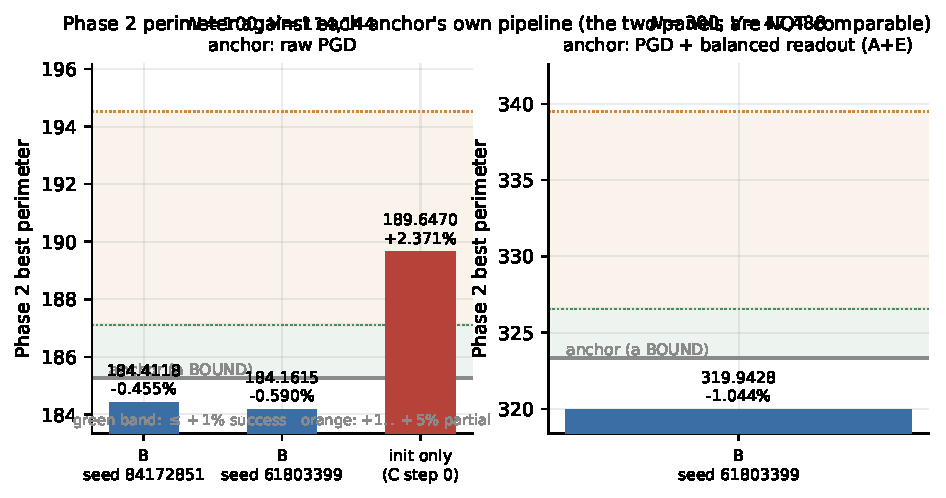
\includegraphics[width=\linewidth]{fig_perimeter.pdf}
\caption{Phase 2 best perimeter against each anchor's own pipeline. \textbf{The two
panels are not comparable and must never be pooled}: the \(N{=}100\) anchor is raw
PGD, the \(N{=}300\) anchor is PGD \emph{plus} the balanced readout, because raw
PGD is not a valid partition at \(N{=}300\).}
\end{figure}

\begin{center}\small
\begin{tabular}{@{}lrrrrrr@{}}
\toprule
run & Phase 1 & speedup & area worst & frag. & Phase 2 best & vs anchor \\
\midrule
\(N{=}100\) s84172851 & \(228\,\mathrm{s}\) & \(210.9\times\) & 0.1504\% & \textbf{0} & 184.4117703525215 (18/20) & \(\mathbf{-0.455\%}\) \\
\(N{=}100\) s61803399 & \(214\,\mathrm{s}\) & \(225.2\times\) & 0.1493\% & \textbf{0} & 184.1614647856558 (19/20) & \(\mathbf{-0.590\%}\) \\
\(N{=}300\) s61803399 & \(248\,\mathrm{s}\) & \(318.8\times\) & 1.4172\% & \textbf{0} & 319.9427628182375 (16/19) & \(\mathbf{-1.044\%}\) \\
\midrule
init only (C step 0) & \(67\,\mathrm{s}\) & --- & 0.1355\% & 0 & 189.6469917457051 (20/20) & \(+2.37\%\) \\
\bottomrule
\end{tabular}
\end{center}

Seed spread at \(N{=}100\) is \(\mathbf{0.136\%}\), which is \(3.3\times\) smaller
than the margin by which the \emph{worse} of the two seeds beats the control. This
is what makes the result scoreable at all: the pre-registration committed that a
spread above \(1\%\) would mean the primary falsifier could not be evaluated at
\(\pm 1\%\) and that a single-seed number would be conflating method difference
with seed noise.

\paragraph{Six constraints on how these numbers may be stated.}
\begin{enumerate}\itemsep2pt
\item \textbf{Never pool the two anchors.} They are different baselines. ``B beats
  the best available PGD pipeline at each \(N\), at equal Phase~2 budget'' is
  valid; ``B beats PGD by \(0.455\text{--}1.044\%\)'' as a trend in \(N\) is not.
\item \textbf{The speedup is for the replaced stage only.} End-to-end, including
  the shared \(30\text{--}40\,\mathrm{min}\) Phase~2, it is \(\approx 23\times\)
  (\(N{=}100\)) and \(\approx 31\times\) (\(N{=}300\)). Against the
  structure-trigger PGD variant (\(34{,}967\,\mathrm{s}\)), the incumbent-best figure is
  \(\approx 153\times\).
\item \textbf{Neither trajectory is a converged optimum.} Both are at the
  documented migration-cycling plateau. An earlier draft said ``B converged where
  the control had not''; the sixth review resumed the control's own Phase~2 for
  \textbf{20 further iterations and found no improvement} (best over all 40 remains
  \(185.2546\) at iterate 20; the extension drifts up to \(\approx 185.30\)). B's
  plateau is simply \(0.455\%\) lower. \emph{That extension is the review's
  measurement and has not been independently reproduced by us.}
\item \textbf{PGD's own seed variance is unmeasured.} Every \(N{=}100\) PGD run
  across both working directories is seed 84172851, and every \(N{=}300\)
  \(\lambda{=}11.5\) run is seed 61803399. Each anchor is a single trajectory.
  ``B beats PGD by more than PGD's own seed lottery'' is \emph{not} established.
\item \textbf{The \(N{=}300\) margin cannot be decomposed, even in principle.} The
  readout costs \(+1.882\%\) in label-boundary length (\(189.7310\) raw \(\to\)
  \(190.7114\) shifted \(\to\) \(193.3024\) repaired, the last being what the
  anchor's Phase~2 consumed). B's raw boundary is \(187.2574\): shorter than the
  repaired labels by \(3.127\%\) \emph{and} shorter than raw PGD's own invalid
  labels by \(1.304\%\) --- the strong form, since imbalance can only make a
  boundary artificially short. So the margin is not merely ``not paying the repair
  bill''. But how much is un-erased repair residue cannot be separated, because
  \textbf{no valid repair-free PGD partition exists at \(N{=}300\)}.
\item \textbf{\(N{=}300\) rests on one Phase-2-scored seed.}
\end{enumerate}

\section{Result 2 --- validity, and which gate actually has content}
\label{sec:gates}

\begin{tcolorbox}[colback=red!3!white, colframe=red!45!black,
                  title={``All three gates pass'' is true and misleading}, fontupper=\small]
An earlier write-up of this result --- ours --- said B's raw labels pass all three
validity gates. Phase~0's own findings say why that is the wrong emphasis:
\begin{itemize}\itemsep1pt
  \item \textbf{Dormant is vacuous} for any balanced-assignment arm. One-hot labels
    give peak density \(1.0\) by construction; the gate cannot fail. The harness
    already emitted \code{vacuous\_for\_arms: True}.
  \item \textbf{Area is near-expected.} Equal area is precisely what B's assignment
    step \emph{optimises}. Passing means the solver converged; Phase~0 defined it
    as the \emph{solver-failure detector}, not a validity test.
  \item \textbf{Connectivity is the only gate genuinely at risk.} Nothing in B
    enforces it, and the source proposal states it is ``not per-step guaranteed''.
\end{itemize}
The defensible claim is narrower and still strong: \textbf{B produces 0 fragmented
cells at \(N{=}300\), where raw PGD produces 2} (with 10 imbalanced cells, worst
\(36.15\%\)) --- which is why PGD's baseline required the balanced readout and B
required nothing.
\end{tcolorbox}

Re-verified through \codefile{testing/check\_fragmentation.py}, which shares no code
with the driver's reporting: all four arm solutions pass, with \textbf{0 cells
having more than one raw component including sub-threshold speckle}.

\paragraph{Robustness.} Three further \(N{=}300\) MBO ladders at seeds 27182818,
13131313 and 84172851 give \textbf{0 fragmented} in every case, with worst area
\(1.2531/1.4467/1.3887\%\) and label boundaries \(186.08/186.55/186.90\) --- all
\emph{shorter} than the scored seed's \(187.2574\). Ladder only, no Phase~2;
\emph{review-produced, not independently reproduced by us}.

\section{Result 3 --- attribution: is this B, or is it C's first step?}
\label{sec:attribution}

B is initialised from one balanced C-scores assignment --- farthest-point seeds,
multi-source Dijkstra, scores \(-d^2\), balanced assignment --- which is literally
approach~C's step~0 \cite{lloyd1982least, aurenhammer1998minkowski,
degoes2012bluenoise}. If MBO barely improved on it, the number in
\S\ref{sec:perimeter} would be a result about C reported under B's name, and
\emph{nothing} in the gate suite would have detected that.

\begin{center}\small
\begin{tabular}{@{}lrrrl@{}}
\toprule
 & Phase 1 & label boundary & Phase 2 best & censored \\
\midrule
init only (C step 0) & \(67\,\mathrm{s}\) & 116.1989 & 189.6469917457051 (20/20) & \textbf{yes} \\
\textbf{B (MBO)} & \(228\,\mathrm{s}\) & 107.6014 & \textbf{184.4117703525215} (18/20) & no \\
control (PGD) & \(48{,}132\,\mathrm{s}\) & 107.3410 & 185.2546144718457 (20/20) & plateaued \\
\bottomrule
\end{tabular}
\end{center}

\[
  \text{P13} \;=\; \frac{189.646992 - 184.411770}{189.646992} \;=\; \mathbf{+2.761\%}
  \qquad\text{against a pre-registered threshold of } 0.3\%.
\]

Two disclosures. The measured \(2.761\%\) is an \textbf{upper bound} on MBO's
contribution, because the init arm is censored: its converged value is
\(\le 189.6470\), and a lower true value shrinks the gap. For attribution to fail
the init would have to reach \(\approx 185.0\) --- another \(\approx 2.5\%\) on a
trajectory gaining \(\approx 0.038\) per iterate and decelerating. And the
init-only control was run on the \emph{finest} mesh, i.e.\ the \emph{strongest}
member of the init family, which biases the test \emph{against} B.

\paragraph{An unflattering free datum on C.} C's step~0 plus Phase~2 lands at
\(+2.37\%\) above the PGD control --- a \textsc{partial} verdict under this
project's own bands --- for \(67\,\mathrm{s}\) of Phase~1. Real C iterates Lloyd and
would improve on this, so it is a \emph{lower bound} on C; but C's starting point
is behind both B and PGD, which is directly relevant to whether C is worth building.
Note also that C minimises a \emph{quantisation} energy, not perimeter; the two
optima coincide only asymptotically and only in the plane
\cite{hales2001honeycomb, gersho1979asymptotically}, and this torus has Gaussian
curvature of both signs.

\section{The mesh ladder, and \(\tau\)}
\label{sec:tau}

\begin{figure}[H]\centering
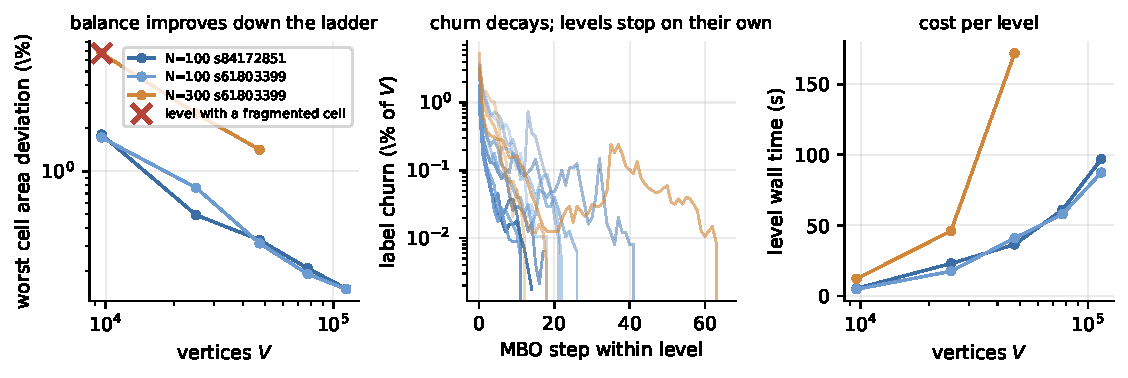
\includegraphics[width=0.95\linewidth]{fig_ladder.pdf}
\caption{Per-level behaviour. Left: worst cell area deviation improves monotonically
down the ladder; the cross marks the one level carrying a fragmented cell. Middle:
label churn decays within every level, so levels terminate on their own rather than
at the iteration cap. Right: cost per level.}
\end{figure}

\(\tau = \min\!\big((c\,h_{\mathrm{mean}})^2,\ (\rho R_{\mathrm{cell}})^2\big)\)
with \(c = 4\) and \(\rho = 1.0\), pinned before any run. \(c=4\) rather than
\(c=2\): the latter is the freeze regime \cite{vangennip2014mean}. The cap is the
over-merge side of a two-sided window, and it binds on exactly one level in use,
\(N{=}300\) level 0.

\begin{figure}[H]\centering
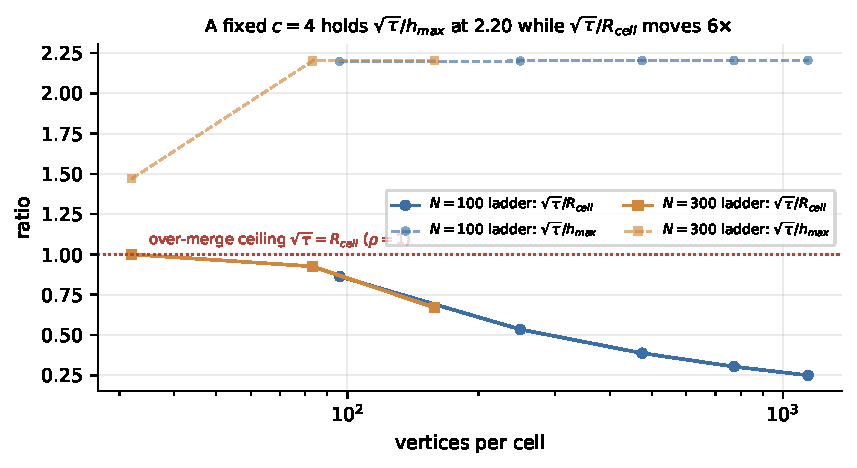
\includegraphics[width=0.9\linewidth]{fig_tau_window.pdf}
\caption{A fixed \(c\) does \emph{not} hold the window. \(\sqrt{\tau}/h_{\max}\)
stays at 2.20 across every level of both ladders while \(\sqrt{\tau}/R_{cell}\)
moves \(6\times\). Reporting on \(h_{\mathrm{mean}}\) alone flatters the coarse
band: this mesh is \(1.81\times\) anisotropic.}
\end{figure}

\section{The headline null: an instrument that detected nothing}
\label{sec:null}

\begin{figure}[H]\centering
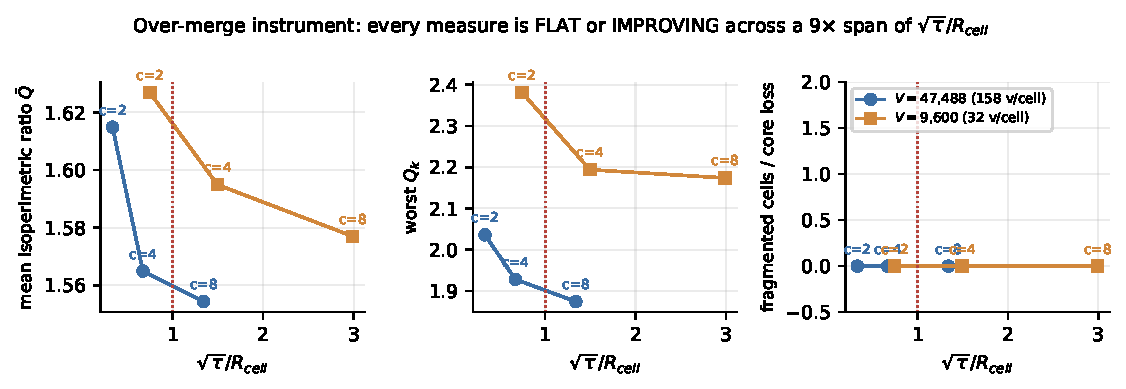
\includegraphics[width=\linewidth]{fig_overmerge_null.pdf}
\caption{Fragmentation, per-cell isoperimetric ratio
\(Q_k = P_k^2/(4\pi A_k)\), and core loss, swept over
\(c \in \{2,4,8\}\) at two resolutions. Every measure is flat or \emph{improving};
none registers an over-merge penalty anywhere, including at
\(\sqrt{\tau}/R_{cell} = 2.99\), three times the pinned cap.}
\end{figure}

Assignment quality \emph{cannot} see over-merging --- the balanced assignment hits
its area target by construction, so a smeared, non-local cell scores as well as a
compact one. (An earlier draft of the plan cited a healthy assignment-quality
fixture as evidence against over-merging; that was a measurement of a different
quantity than the claim it supported, and it was withdrawn.) So three geometry
instruments were built. Across a \(9\times\) span of \(\sqrt{\tau}/R_{cell}\) and
two levels differing \(5\times\) in resolution, \textbf{not one of them registered
anything}: core loss and fragmentation are 0 in all six configurations, and
compactness moves monotonically the \emph{other} way.

The instruments are demonstrably \emph{responsive} --- \(\bar{Q}\) moves 3.8\%,
\(Q_{\mathrm{worst}}\) 8\%, boundary length 1.9\% --- they simply move toward
improvement. What is established is therefore that \textbf{no damage is
detectable}, \emph{not} that over-merging cannot occur.

\begin{tcolorbox}[colback=yellow!6!white, colframe=orange!60!black,
                  title={Standing limit}, fontupper=\small]
The \(\rho\) question is \textbf{open}, and no future claim about \(c\) or \(\rho\)
may lean on this report's evidence in either direction. The cap was retained
because it is pre-registered and because it biases \emph{against} B --- it lowers
\(c\) to 2.68 at \(N{=}300\) level 0, and \(c{=}2\) measures worse than \(c{=}4\).
That is a discipline argument, not an empirical one. \textbf{Named follow-up:}
\(c{=}8\) showed no penalty on any instrument \emph{and} a \(0.33\%\) shorter
starting boundary --- a third of the entire \(+1\%\) success bar --- so the cap may
be costing perimeter for no measured benefit. That is a separate arm, scored
through the same harness.
\end{tcolorbox}

\section{Why there is no exactly-monotone energy, and what is gated instead}
\label{sec:descent}

Esedo\u{g}lu--Otto monotonicity is a minorise--maximise argument requiring (i)~the
same symmetric positive semi-definite form in the energy and in the assignment
objective, and (ii)~an \emph{exact} assignment. \textbf{Both fail here, for
independent reasons.} The theorem's object is \(M A_\tau = M(M+\tau K)^{-1}M\),
symmetric PSD; our step maximises \(\langle \chi', D y\rangle\) with
\(D = \operatorname{diag}(v)\) \emph{lumped}, and \(D A_\tau\) is not symmetric.
And Jacobs, Merkurjev and Esedo\u{g}lu obtain a theorem because Bertsekas'
auction is exact,
whereas \code{solve\_dual\_offsets} is subgradient ascent returning its best
iterate. \textbf{This is the price of a substitution made deliberately in Phase~0}
--- where Sinkhorn \cite{cuturi2013sinkhorn} and auction were both measured and
both lost to the incumbent on assignment quality --- paid here rather than there.

What survives needs neither concavity nor exactness. Since
\(\omega'(i) = \arg\max_k [y_{ik} + \psi_k]\), multiplying the pointwise optimality
by \(v_i > 0\) and summing gives
\[
  \boxed{\ \langle \chi', D y\rangle - \langle \chi, D y\rangle
    \;\ge\; \sum_k \psi_k\,(T_k - T'_k)\ }
\]
whose right-hand side is exactly the slack that inexactness costs; it vanishes at
perfect balance. Measured slack runs \(1.7\times10^{-4}\) to
\(5.5\times10^{-3}\) --- five to seven orders of magnitude above the
\(10^{-9}\) tolerance an earlier draft proposed for energy monotonicity, so that
tolerance was never defensible. \textbf{Real \(E_\tau\) increases do occur} (4 of
96 active steps at \(N{=}300\)), and gate G4 therefore gates the inequality, whose
measured violation is \(\le 6.13\times 10^{-8}\), while \(E_\tau\) is reported as a
descriptive trend only.

\section{Predictions, and what they caught}
\label{sec:predictions}

\begin{figure}[H]\centering
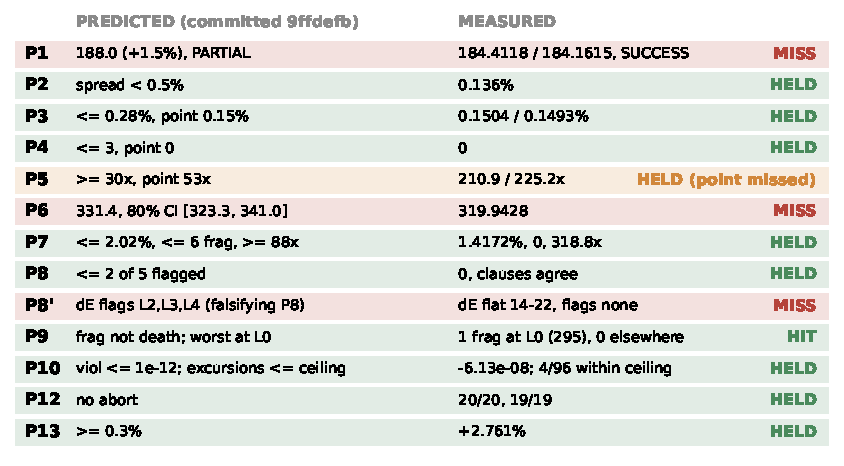
\includegraphics[width=\linewidth]{fig_predictions.pdf}
\caption{Thirteen predictions committed in \code{9ffdefb} at 16:53, before the first
scored run at 17:34:11.}
\end{figure}

\paragraph{P1 and P6 missed, and P1's \emph{reasoning} is refuted.} The rationale
was that B sees perimeter only through a coarse-\(\tau\) surrogate while PGD saw
the actual energy for \(13.4\,\mathrm{h}\). B also \emph{enters} Phase~2 from a
\(0.243\%\) \emph{longer} boundary than the control and still finishes ahead --- a
genuine crossover, so the advantage is not initial geometry. That it is
combinatorial is a hypothesis consistent with these data, not established by them.
P6 missed worse: its \(80\%\) interval's lower bound was the anchor itself, so
essentially no probability was assigned to B beating PGD\,+\,A\,+\,E at
\(N{=}300\).

\paragraph{P8\('\) missed and invalidated its own model.} It predicted, from a
log-linear interpolation of \(\Delta E/\text{tail}\) in the freeze ratio
\(c/c_{\mathrm{lo}}\), that levels 2--4 would be flagged pinned. Measured,
\(\Delta E/\text{tail}\) is \emph{flat} across the ladder --- 15.76, 21.62, 15.11,
14.22, 16.49 against a threshold of 79.25 --- and level 4, sitting exactly at
\(c/c_{\mathrm{lo}} = 0.999\), scores 16.49 where the model demanded \(\approx 260\).
The freeze ratio does not predict pinning here.

\section{The sixth artefact --- and it is ours}
\label{sec:artefact}

Report~07 catalogued five occasions on which a measurement artefact was read as a
result about the method. This is the sixth, and it was produced in this work.

The plan asserted \textbf{``0 fragmented at every level''} and, on that basis,
scored P9 --- which predicted over-merge would appear as fragmentation rather than
cell death, worst at level 0 --- as \textsc{untestable}, ``the predicted phenomenon
never occurred''. \textbf{Until the sixth review, \code{LevelReport} carried no
connectivity field at all.} Per-level fragmentation had never been computed. The
claim was an inference presented as a result, and it was false.

With the instrument added and the \(N{=}300\) ladder re-run to a bit-exact
reproduction (worst areas \(6.7063/2.5394/1.4172\%\), steps \(16/21/66\), boundary
\(187.2574\)):

\begin{center}\small
\textbf{level 0: 1 fragmented cell (cell 295). Levels 1 and 2: 0. No cell death.}
\end{center}

The phenomenon occurred, at exactly the level P9 named, in exactly the form P9
predicted. \textbf{P9 is a hit, not untestable} --- ``untestable'' had absorbed a
correct prediction on the strength of a measurement never taken. The stray is
healed by level 1's MBO run, which is direct evidence for the mechanism the
taxonomy predicted: stray islands are perimeter-inefficient and shrink under
curvature flow, the opposite dynamic to the discrete-area trim that manufactured
them.

The fix is instrumentation --- \code{run\_gates} per level, seconds of cost, now
committed --- not a resolution to be careful.

\section{Result 5 --- \(N{=}400\), \(500\), \(750\): existence where the anchor cannot exist}
\label{sec:n400}

The three results above are all \emph{margins}: B against a control, at a pinned
Phase~2 budget. That design has a ceiling built into it. It can only be run where
a control exists, and the control is the method whose cost is the reason B was
built. Pushed far enough in \(N\), the comparison stops being expensive and starts
being impossible.

\(N{=}400\), \(500\) and \(750\) are past that point, and this section reports
them as what they are: \textbf{existence-and-validity} results with no anchor, no
margin, and no comparison of perimeters. All three ran in the driver's exploratory
\code{-{}-config} mode, where the mesh-match assertion is skipped because there is
nothing to match. \(N{=}500\) deliberately reuses \(N{=}400\)'s ladder unchanged,
which converts the \(\sqrt{N}\) argument below from a single check into a
three-point one; \(N{=}750\) could not, for a reason that is itself a result
(\S\ref{sec:ladder750}).

\subsection*{The results}

\(N{=}400\) and \(N{=}500\) run to \(V = 114{,}144\); \(N{=}750\) runs to
\(V = 158{,}260\). All three validity gates pass on the \emph{raw} labels at every
\(N\), re-verified with \codefile{testing/check\_fragmentation.py} independently
of \code{arm\_report.yaml}:

\begin{center}\small
\begin{tabular}{@{}lrrr@{}}
\toprule
 & \(N{=}400\) & \(N{=}500\) & \(N{=}750\) \\
\midrule
Phase~1 wall & \(920\,\mathrm{s}\) & \(1{,}322\,\mathrm{s}\) & \(3{,}614\,\mathrm{s}\) \\
dormant & 0 / 0 & 0 / 0 & 0 / 0 \\
area imbalance (bar) & 0, \(\mathbf{0.7773\%}\) (1.1214) & 0, \(\mathbf{1.0993\%}\) (1.4017) & 0, \(\mathbf{1.2569\%}\) (1.5165) \\
connectivity & \(\mathbf{0}\) & \(\mathbf{0}\) & \(\mathbf{0}\) at \emph{every} level \\
Phase~2 perimeter & \(\mathbf{368.6603}\) & \(\mathbf{412.1138}\) & \(\mathbf{504.9214}\) \\
 & (it.\ 19/20) & (it.\ 10/20) & (it.\ 14/20) \\
variable points & 29{,}287 & 32{,}704 & 47{,}088 \\
max area violation & \(8.18\mathrm{e}{-7}\) & \(1.10\mathrm{e}{-6}\) & \(4.68\mathrm{e}{-7}\) \\
\bottomrule
\end{tabular}
\end{center}

All three Phase~2 constraint residuals are converged to tolerance, so the
partitions are genuinely equal-area rather than approximately so, and the
\(N{=}500\) and \(N{=}750\) bests are \emph{mid-trajectory} --- not censored; both
descend and then oscillate in the migration-cycling plateau. All three
deliverables are exported with \code{finalised=True}.

\subsection*{The \(\sqrt{N}\) cross-check, three points}

Not a gate, and the sharpest instrument available in the absence of an anchor. On
a \emph{fixed} mesh total perimeter should scale as \(\sqrt{N}\); all three runs
below sit on the same \(V = 114{,}144\) mesh, so the comparison is free of any
refinement effect. \(N{=}500\) was given \(N{=}400\)'s ladder unchanged precisely
to make this test available, and its predicted value was recorded in
\codefile{parameters/torus\_500part\_mbo.yaml} \emph{before} the run.

\begin{center}\small
\begin{tabular}{@{}lrrr@{}}
\toprule
 & predicted & measured & deviation \\
\midrule
\(N{=}100 \to N{=}400\) & \(368.8236\) & \(368.6603\) & \(-0.044\%\) \\
\(N{=}400 \to N{=}500\) & \(412.1748\) & \(\mathbf{412.1138}\) & \(\mathbf{-0.015\%}\) \\
\(N{=}100 \to N{=}500\) & \(412.3573\) & \(412.1138\) & \(-0.059\%\) \\
\bottomrule
\end{tabular}
\end{center}

Three independent runs at three values of \(N\) agree with the scaling to better
than \(0.06\%\). All three deviations are negative, which is a consistent slight
shortfall rather than scatter; with three points we do not attempt to say why.

\(N{=}750\) is \emph{not} in that table, because it runs on a different mesh and
the test is only sharp at fixed \(V\). Recorded for completeness and scored
against nothing: the fixed-mesh value implied by \(N{=}500\) is \(504.7342\) and
the measurement is \(504.9214\), \(+0.037\%\). Two points worth stating plainly.
The magnitude is small, but the \emph{sign} is opposite to all three fixed-mesh
checks, and the pre-registered expectation in
\codefile{parameters/torus\_750part\_mbo.yaml} was that a finer mesh should land
slightly \emph{below} --- so the stated direction was wrong. Nothing is concluded
from a single unscored point; it is noted so the error is on the record.

\subsection*{The ladder had to change at \(N{=}750\), and the diagnostics said so first}
\label{sec:ladder750}

Every earlier config began at \(100\times96\). At \(N{=}750\) that rung is
unusable, and this is visible \emph{before} running: it gives 12.8 verts/cell and
\(\sqrt{\tau}/h_{\max} = 0.929\) against a local non-freeze threshold of
\(0.964\) --- a ratio of \(\mathbf{0.964}\), \textbf{below 1}, so the
coarse-triangle band cannot move at all. Every measured run had been above 1 at
every level (\(N{=}400\) min 1.049, \(N{=}500\) min 1.067).

The mechanism is a squeeze that tightens with \(N\): more cells means smaller
cells, the over-merge cap holds \(\sqrt{\tau} \le R_{\mathrm{cell}}\), so the
diffusion length shrinks --- while the coarse mesh's triangles do not. Past some
\(N\) the diffusion no longer reaches across one triangle and the level freezes.
\textbf{The remedy is the ladder, not \(\tau\)}: raising \(\tau_c\) walks toward
the over-merge wall on the other side of the same two-sided window. The config
therefore keeps levels 1--5 verbatim and drops the dead rung, running
\(162\times154 \to 410\times386\). Every level then sits at ratio \(\ge 1.131\),
and the finest level's margin (1.131) is better than \(N{=}500\)'s (1.109) and
\(N{=}400\)'s (1.049), both of which ran clean.

It worked, and it bought something beyond avoiding the freeze: \(N{=}750\) is the
first high-\(N\) run with \textbf{zero fragmented cells at every level}, where
\(N{=}300\) and \(N{=}500\) each produced one at level 0 that later levels had to
heal. Starting at 33 verts/cell instead of 12.8 or 19.2 removes the defect rather
than repairing it.

\subsection*{Two mechanisms recur at a third \(N\)}

Neither is new; both were predicted or observed earlier, and \(N{=}500\) is an
independent occasion for them to fail.

\textbf{Level-0 fragmentation, healed by level 1.} \(N{=}500\) level 0 produces
one fragmented cell (323) and level 1 has none --- exactly the pattern
\S\ref{sec:artefact} recorded at \(N{=}300\) (cell 295), and the mechanism the
taxonomy predicts: stray islands are perimeter-inefficient and shrink under
curvature flow. \(N{=}400\) shows none at any level. This is visible only because
the per-level instrument now exists; it is the same claim that was once asserted
with nothing measuring it.

\textbf{The over-merge null holds.} At \(N{=}500\) the cap binds on two levels and
\(\sqrt{\tau}/R_{\mathrm{cell}}\) is at its ceiling there, yet the instrument
reports \(\text{core loss} = 0\) at every level, \(q_{\mathrm{worst}}\) falling
\(2.95 \to 1.81\) down the ladder, and \(q_{\mathrm{mean}}\) in
\(1.54\text{--}1.61\) against \(N{=}400\)'s \(1.56\text{--}1.57\). A third \(N\),
a tighter cap, and the same null of \S\ref{sec:null}. Still undetected rather
than excluded.

\subsection*{The mesh-matched companions, and a level 0 below the freeze threshold}
\label{sec:meshmatched}

The runs above each use the finest ladder their \(N\) can support, so \(N{=}750\)
and \(N{=}1000\) end at \(V{=}158{,}260\) and \(209{,}568\) while every earlier
deliverable ends at \(114{,}144\). The exported partition carries the Phase~1
mesh, so a downstream study measuring per-cell quantities cannot compare across
\(N\) when the mesh changes underneath it. Both were therefore re-run on the
\emph{common} mesh --- and not merely to the same endpoint. Matching only the
endpoint would be a different algorithm: in a multi-level scheme the coarse levels
do the structural work and the fine levels refine it. The companions use the
\textbf{identical ladder, seed and \(\tau\) constants as the \(N{=}400/500\)
configs}, changing only \code{n\_partitions}.

That forces \(100\times96\) as the base rung, where the two large \(N\) sit
\emph{below} the freeze threshold --- a regime no previous run had entered:

\begin{center}\small
\begin{tabular}{@{}lrrrrl@{}}
\toprule
 & level-0 ratio & v/cell & level-0 floor & final worst & bar \\
\midrule
\(N{=}750\)  & \(0.964\) & 12.8 & \(12.4997\%\) & \(\mathbf{1.6928\%}\) & \(2.1026\%\) \\
\(N{=}1000\) & \(0.897\) & \phantom{0}9.6 & \(16.6663\%\) & \(\mathbf{2.2560\%}\) & \(2.8035\%\) \\
\bottomrule
\end{tabular}
\end{center}

\textbf{Both pass all three gates: 0 dead, 0 weak, 0 imbalanced, 0 fragmented.}
So a sub-threshold level 0 is \emph{survivable} under B. Three observations, the
first two of which were not predicted:

\textbf{(1) It is a partial, not total, freeze --- and it costs real work.}
Scoring each level by the fraction of the improvement available to it that it
actually captured (its floor being the target it cannot pass), level 0 captures
\(18\%\) at \(N{=}750\) and \(26\%\) at \(N{=}1000\), where every healthy level
in both runs captures \(55\text{--}89\%\). About a third of normal. This matches
the mechanism: the diffusion reaches past the mean edge but not the largest, so
fine-triangle regions evolve while the anisotropic coarse band does not.

\textbf{(2) The freeze ratio does not predict how much a sub-threshold level
accomplishes.} \(N{=}750\) has the \emph{better} ratio (0.964 vs 0.897) and more
verts/cell, and was predicted to fare at least as well; it captured \emph{less}
(18\% vs 26\%). With two points no mechanism is offered, but the ratio alone is
evidently not the controlling variable below 1.0.

\textbf{(3) The damage is manufactured at level 0 and fully healed.} Level 0
produced 2 fragmented cells at \(N{=}750\) and 3 at \(N{=}1000\) --- more than any
run above threshold --- and the chains clear completely:
\(2 \to 0 \to 0 \to 0 \to 0\) and \(3 \to 2 \to 1 \to 0 \to 0\). This is the
distinction from PGD, where \codefile{docs/experiments/06-subfloor-ladder/}
measured a starved level 0 leaving a \emph{permanent} runt (46.80\% \(\to\)
15.92\% across 37\(\times\) more vertices). Under B the same insult is transient.

\subsection*{Two properties of the common mesh worth recording}

\textbf{Worst-cell error saturates at \(\approx 1.61\times\) the granularity
floor.} On the fixed \(V{=}114{,}144\) mesh:

\begin{center}\small
\begin{tabular}{@{}lrrr@{}}
\toprule
 & worst & floor & ratio \\
\midrule
\(N{=}400\)  & \(0.7773\%\) & \(0.5607\%\) & \(1.386\) \\
\(N{=}500\)  & \(1.0993\%\) & \(0.7009\%\) & \(1.568\) \\
\(N{=}750\)  & \(1.6928\%\) & \(1.0513\%\) & \(\mathbf{1.610}\) \\
\(N{=}1000\) & \(2.2560\%\) & \(1.4017\%\) & \(\mathbf{1.609}\) \\
\bottomrule
\end{tabular}
\end{center}

It rises and then plateaus. If that holds, quality on a fixed mesh is predictable
from the mesh alone --- worst cell \(\approx 1.61 \times\) granularity, which
scales as \(N/V\) --- so a mesh can be sized for a target area error without
running anything. Four points and no mechanism: a pattern, not a law.

\textbf{A coarser mesh under-measures perimeter.} \(N{=}1000\) reads
\(583.1417\) at \(V{=}114{,}144\) against \(583.2558\) at \(209{,}568\),
\(-0.020\%\). The direction is not noise: a boundary represented by fewer, longer
straight segments is a shorter approximation to the same curve, so the coarse
value is an underestimate and the finer one is closer to the truth. Small, but it
biases any perimeter-derived quantity systematically with \(N\) when the mesh is
held fixed --- which is the price of holding it fixed.

\textbf{Equal-area accuracy of the exported geometry is unaffected by any of
this.} The percentages above are Phase~1's \emph{discrete} winner-take-all
imbalance and do not survive into the export; Phase~2 equalises the actual
geometric areas. Measured on the exported best iterates, the worst cell is off
target by \(0.0014\%\) (\(N{=}400\)), \(0.0023\%\) (\(500\)), \(0.0272\%\)
(\(750\)) and \(0.0127\%\) (\(1000\)) --- the two mesh-matched runs are the
loosest of the set, as fewer verts/cell would predict, and all four are
negligible.

\subsection*{Why the missing anchor is the finding}

The obvious objection is that a result without a baseline is weak. Here it is the
reverse, and the reason is measurable rather than rhetorical. Compare at the
\textbf{matched} finest mesh \(V = 114{,}144\) --- the same mesh, so no
refinement effect enters:

\begin{center}\small
\begin{tabular}{@{}lrr@{}}
\toprule
 & PGD, \(N{=}300\) & B, \(N{=}400\) \\
 & \code{run\_20260808\_191030} & \code{arm\_mbo\_20260820\_133709} \\
\midrule
Phase~1 wall & \(206{,}344\,\mathrm{s}\) \((57.3\,\mathrm{h})\) & \(\mathbf{920\,\mathrm{s}}\) \\
dead / weak & 0 / 0 & 0 / 0 \\
area imbalance & \textbf{3 imbalanced, worst \(24.81\%\)} & 0, worst \(\mathbf{0.78\%}\) \\
fragmented & \textbf{2} & \(\mathbf{0}\) \\
valid on raw labels? & \textbf{no} --- requires the readout & \textbf{yes} \\
\bottomrule
\end{tabular}
\end{center}

On the identical mesh, with \emph{one hundred fewer cells}, the incumbent took
\(\mathbf{224\times}\) the wall time and failed two of the three gates. Requiring
a PGD anchor at \(N{=}400\) therefore asks the incumbent to do precisely the thing
whose absence motivated B. The honest claim needs no margin:

\begin{quote}
Approach~B produces a valid, equal-area, fully connected 400-cell partition on a
114{,}144-vertex torus from 15 minutes of Phase~1, in a regime where the incumbent
has already ceased to produce valid partitions at \(N{=}300\) on the same mesh.
\end{quote}

\subsection*{What this section does \emph{not} claim}

The \(-0.455\%\) and \(-1.044\%\) margins of \S\ref{sec:perimeter} are not
extended to \(N{=}400\) or \(N{=}500\), and no perimeter here is compared against
PGD. The
matched-mesh table above is a statement about \emph{validity and cost}, both
measured on both sides at the same \(V\); it is not a perimeter comparison, and
the two must not be blurred. The \(\sqrt{N}\) check is B against B, so it tests
internal consistency, not correctness against an independent method: three runs
agreeing on a scaling law they all obey would not detect an error common to all
three. And \(N{=}500\) reuses \(N{=}400\)'s ladder and seed, so the two are not
independent in the mesh or the initialisation, only in the run.

\subsection*{The cost centre has moved --- and it is not the solver}

Phase~2 took \(7{,}326\,\mathrm{s}\), \(8{,}829\,\mathrm{s}\) and
\(\mathbf{18{,}323\,\mathrm{s}}\) (5.09\,h) at \(N{=}400/500/750\), against
Phase~1's 920\,s, 1{,}322\,s and 3{,}614\,s. The stage this report replaces is
therefore \(11\%\), \(13\%\) and \(16.5\%\) of end-to-end cost --- the last rising
only because \(N{=}750\) was given an extra ladder level. The
\(211\text{--}319\times\) of \S\ref{sec:perimeter} was always a statement about
the replaced stage; past \(N{=}400\) the remainder dominates.

The \(N{=}500\) and \(N{=}750\) campaigns were run with \code{-{}-profile}, and
the breakdown is not what the forward plan assumed. \textbf{The IPOPT solver
accounts for \(5.2\%\) of the campaign at \(N{=}500\) and \(3.6\%\) at
\(N{=}750\)} --- a \emph{shrinking} share of a growing problem. At both, IPOPT
runs 201 solver iterations per topology iteration, hitting
\code{max\_opt\_iter: 200} every time, and the internal callback split is
essentially identical (Hessian \(40.4\%\) vs \(40.7\%\) of solver time). So
\(95\text{--}96\%\) of Phase~2 is spent \emph{outside} \code{optimize()}: contour
rebuild, Steiner setup, migration detection and checkpoint export with its
roundtrip verification. \textbf{We establish the solver's share, not the
composition of the remainder} --- decomposing that is the measurement
\codefile{docs/plans/PUBLICATION\_READINESS\_PLAN.md} Phase~4 should now make,
in place of its original premise that the exact-Hessian path was the target.

\textbf{Phase~2 also scales superlinearly in variable points, close to
quadratically.} Campaign wall against variable-point count:

\begin{center}\small
\begin{tabular}{@{}lrrrl@{}}
\toprule
 & variable points & wall & s/VP & exponent \\
\midrule
\(N{=}400\) & 29{,}287 & \(7{,}326\,\mathrm{s}\) & 0.250 & \\
\(N{=}500\) & 32{,}704 & \(8{,}829\,\mathrm{s}\) & 0.270 & 1.69 \\
\(N{=}750\) & 47{,}088 & \(18{,}323\,\mathrm{s}\) & 0.389 & \textbf{2.00} \\
\bottomrule
\end{tabular}
\end{center}

\(N{=}1000\) has since been measured and extends the table: 62{,}472 variable
points, \(29{,}946\,\mathrm{s}\), \(0.479\,\mathrm{s}\)/VP, exponent
\(\mathbf{1.74}\). \textbf{An earlier version of this paragraph called the trend
``superlinear and \emph{steepening}''; the fourth point refutes the second half}
--- the exponents run \(1.69 \to 2.00 \to 1.74\), so 2.00 was an excursion, not a
trend. The defensible statement is \emph{superlinear, exponent \(\approx\)
1.7--2.0, with no evident trend}, which is a better outlook than the wording it
replaces because it means the cost is not accelerating away.

One cleaner comparison is now available. \(N{=}750\) and \(N{=}1000\) both have
mesh-matched companions on \(V{=}114{,}144\) (\S\ref{sec:meshmatched}), giving the
first pair measured at \emph{fixed} mesh: 39{,}704 VPs / \(12{,}908\,\mathrm{s}\)
and 45{,}859 VPs / \(18{,}138\,\mathrm{s}\), an exponent of \(\mathbf{2.36}\) ---
steeper than any of the mixed-mesh figures, which suggests part of what was being
attributed to variable-point count was a mesh effect. Two points, so this is a
flag for a third measurement rather than a result. Either way Phase~2 is the
binding constraint on \(N\).

\emph{Measurement note.} The \(N{=}750\) mesh-matched campaign was launched twice
--- the first attempt wrote iterate 1 and stopped --- leaving 21 iterate files,
two of them bit-identical copies of iteration 1. Its wall time must be taken from
the \emph{second} launch (\(12{,}908\,\mathrm{s}\)); measuring from the campaign
directory spans the aborted attempt and reads \(14{,}021\,\mathrm{s}\), \(9\%\)
high. It is the only campaign of the ten with more than one launch.

\begin{tcolorbox}[colback=red!3!white, colframe=red!45!black,
                  title={A reporting trap in \code{timing\_profile.yaml}},
                  fontupper=\small]
The Phase~2 profile's \code{summary.total\_wall\_s} is \(459.27\,\mathrm{s}\)
while the campaign took \(8{,}829\,\mathrm{s}\). The field accumulates only time
inside \code{optimizer.optimize()}; everything else in the loop is outside it. A
\(\mathbf{19\times}\) under-report if read as campaign wall --- the same class of
trap as \code{run\_time\_seconds} in the Phase~1 metadata, which under-reports by
\(3.6\times\) and is already documented. Campaign wall must be taken from the
iterate timestamps.
\end{tcolorbox}

Two scaling consequences worth recording. The \(\tau\) over-merge cap binds on
\emph{two} levels at both \(N\) (against one at \(N{=}300\) and none at
\(N{=}100\)) as cells shrink relative to the coarse mesh. And the
vertex-granularity floor has risen from \(0.5607\%\) to \(0.7009\%\), pushing the
worst cell from \(1.39\times\) to \(1.57\times\) that floor against a \(2\times\)
bar --- so the finest mesh will have to grow before the bar is reached, and that
raises Phase~2, which is now the expensive half.

\section{Threats to validity that no instrument here addresses}
\label{sec:threats}

\begin{enumerate}\itemsep2pt
\item \textbf{PGD's seed variance} (\S\ref{sec:perimeter}, constraint 4). Both
  anchors are single trajectories; the corpus was enumerated across \emph{both}
  working directories, since \code{results/} is gitignored and each worktree has
  its own.
\item \textbf{Over-merging} (\S\ref{sec:null}). Not excluded, merely undetected.
\item \textbf{Phase 2 budget as a confound.} B may start from geometry that lets
  Phase~2 converge \emph{within} a budget PGD cannot use as well. The 40-iteration
  control extension argues against this, but is review-produced.
\item \textbf{Same-machine identity} of the July control and the August arms is
  consistent with the recorded hardware but is not stamped in run metadata.
\item \textbf{\(N{=}1000\)} is untouched. Nothing here establishes that B's
  behaviour extrapolates.
\end{enumerate}

\section{Conclusions}
\begin{enumerate}\itemsep2pt
\item B replaces Phase~1 at \(211\text{--}319\times\) less wall time in the replaced
  stage and reaches a \emph{shorter} Phase~2 perimeter than the best available PGD
  pipeline at both \(N\), at equal Phase~2 budget.
\item Its raw labels are connected at both \(N\) --- the one validity gate B could
  have failed --- so the readout and repair stages are unnecessary for B.
\item The advantage is attributable to the MBO dynamics, not to the balanced
  geodesic initialisation, by \(+2.761\%\) against a \(0.3\%\) threshold.
\item Three pre-registered predictions missed, all in B's favour, and one was
  initially mis-scored in B's \emph{dis}favour by an instrument that did not exist.
\end{enumerate}

\section*{Provenance of the two closest references}
Both papers are held at \codefile{docs/papers/}. Authors, titles and versions are
now \textbf{verified against their title pages}:
\cite{hu2024iterative} is Shilong Hu, Hao Liu and Dong Wang (v1, 25 May 2024) ---
an earlier draft of this report guessed two of the three given names wrongly, from a
secondary description --- and \cite{bogosel2021longest} is Beniamin Bogosel and
Edouard Oudet (v2, 7 June 2021).

The scope characterisation is now partly checked directly rather than taken on
trust: \cite{hu2024iterative} states in its abstract that it treats the
\emph{longest} minimal length partition problem by Gaussian convolution with
auction dynamics and threshold dynamics, on \(128\times128\) and
\(256\times256\) grids in 2D and 3D, and its full text contains \textbf{zero}
occurrences of ``manifold'', ``Riemannian'' or ``torus'';
\cite{bogosel2021longest} states in its abstract that it seeks the set maximizing
the perimeter of the least-perimeter partition and uses capacity-constrained
Voronoi diagrams as \emph{initialization}, with 44 occurrences of ``convex'' and
2 of ``manifold''. \textbf{What remains second-hand} is the reading of their full
numerical sections; the author has read the title pages, abstracts and these
keyword counts, not the papers end to end.

Volume and page numbers throughout \codefile{docs/math/shared/references.bib}
carry an upstream note that they should be checked against published sources
before external distribution. That note still stands for the other 28 entries,
none of which this report verified.

\section*{Related documents}
\begin{itemize}\itemsep1pt
\item Plan, pre-registration and full correction history:
  \codefile{docs/plans/PHASE1\_BC\_REPLACEMENT\_PLAN.md}
\item Taxonomy: \codefile{docs/reference/PHASE1\_HIGHN\_APPROACHES\_ABCDE.md}
\item The instrument this report is scored through: \codefile{docs/experiments/07-phase0-shared-harness/}
\item The gap B makes vacuous: \codefile{docs/reference/winner\_take\_all\_partition\_gap.md}
\end{itemize}

\bibliographystyle{plain}
\bibliography{../../math/shared/references}

\end{document}
